\documentclass{beamer}

\usepackage{color}
\usepackage{amssymb}
\usepackage[latin1]{inputenc}
\usepackage{afterpage}
\usepackage[T1]{fontenc}
\usepackage{amsfonts}
\usepackage{mathtools}
\usepackage[italian]{babel}
\usepackage{graphicx}
\usepackage{amsmath}
\usepackage{amsfonts}
\usepackage{amssymb}
\usepackage{amsthm}
\usepackage{tikz}
\usetikzlibrary{arrows}


\mode<presentation>
{
  \usetheme{Madrid}
  \setbeamercovered{transparent}
  \usecolortheme{wolverine}
\usefonttheme{professionalfonts}

}



\usepackage{times}
\usepackage[T1]{fontenc}

\newcommand{\argmax}[1]{\underset{#1}{\operatorname{arg}\,\operatorname{max}}\;}
\def\R{\mathbb{R}}
\def\e{\varepsilon}
\def\l{\lambda}
\def\bh{\textbf{h}}
\def\bd{\textbf{d}}
\def\bx{\bar{x}}
\def\boldx{\textbf{x}}

\title{Progetto Finale \\
 di Statistica Computazionale} 

\author{Davide Torlo \& Luca Venturi}

\institute[UniTs]
{Universit� degli Studi di Trieste\\
Dipartimento di Matematica e Geoscienze}


\date[21 Gennaio 2016]
{21 Gennaio 2016}


\begin{document}

\begin{frame}
  \titlepage
\centering 
{\small {Professore\\ Prof. Luca Bortolussi}}
\end{frame}

\begin{frame}{Sintesi}
  \tableofcontents
  % You might wish to add the option [pausesections]
\end{frame}

\section{Task 1 - Regressione}

\begin{frame}{Task 1 - Regressione}
\begin{itemize}
\item{Dataset composto da 99 parametri di 1994 citt� americane.}
\vspace{ 3mm}\\
\item{La funzione dataci � il tasso di criminalit� nelle singole citt�.}
\vspace{ 3mm}\\
\item{Oltre ai 99 parametri, un centinaio di citt� avevano altri 20 parametri.}
\vspace{ 3mm}\\
\item{Obiettivo: creare un modello di regressione che preveda il tasso di criminalit� in altre citt�.}
\end{itemize}
\end{frame}

\begin{frame}{Regressione - Preprocessing}
\begin{itemize}
\item{Abbiamo usato i processi Gaussiani per costruire un modello di regressione.}\vspace{3mm}
\item{Per preprocessare i dati abbiamo provato a rinormalizzarli (erano forniti tutti tra $0$ e $1$) su un compatto di $\mathbb{R}$ centrato in $0$, ma senza ottenere grandi risultati.}\vspace{3mm}
\item{Fondamentale � stata la riduzione di dimensione. Usando la PCA siamo passati a dimensione dalle 2 alle 30 a seconda degli algoritmi usati.}

\end{itemize}
\end{frame}

\begin{frame}{Regressione - Homemade GP Regression}
\begin{itemize}
\item{Abbiamo usato l'algoritmo dei processi Gaussiani visto a lezione.}\vspace{3mm}
\item{Il primo problema trovato � stato quello di invertire la matrice di Gram $K$ con numeri di dati troppo elevati.}\vspace{3mm}
\item{Quindi abbiamo diviso il training set, in diversi training set da circa 100/200 dati ciascuno.}\vspace{3mm}
\item{Per ognuno di questi avevamo parametri da ottimizzare.}

\end{itemize}
\end{frame}


\begin{frame}{Regressione - Homemade GP Regression}
\begin{itemize}
\item{Per ogni training set usato abbiamo usato dei validation set per ottimizzare i parametri di lengthscale, amplitude e noise che usa il nostro metodo.}\vspace{3mm}
\item{Per far ci� abbiamo usato la function \texttt{fmincon} di Matlab su una funzione che prende in ingresso i parametri e restituisce l'errore quadratico medio dei punti del validation set dalla regressione stimata.}\vspace{3mm}
\item{Con i parametri ottenuti abbiamo fatto la regressione su nuovi punti di test e infine mediato sulle diverse soluzione ottenute dai diversi training set.}

\end{itemize}
\end{frame}


\begin{frame}{Regressione - Homemade GP Regression}
\begin{itemize}
\item{Questo metodo porta con se un po' di problemi.}\vspace{3mm}
\item{Primo di tutti ottiene dei risultati non molto ottimali, in quanto il massimo che siamo riusciti a raggiungere � stato una media quadratica dell'errore di $0.6532$ (con $t\in [0,1]$) e con varianza molto elevata (varianza media attorno a $1$.)}\vspace{3mm}
\item{Inoltre i parametri ottimali trovati da Matlab sono davvero molto sensibili ai dati iniziali e al training set.}\vspace{3mm}
\item{Ci� ci fa supporre che la funzione abbia tanti minimi locali e che sia facile non trovare il minimo assoluto.}
\end{itemize}
\end{frame}

\begin{frame}{Regressione - Matlab GP Regression}
\begin{itemize}
\item{Abbiamo provato ad usare la funzione di Matlab che implementa la regressione con processi Gaussiani.}\vspace{6mm}
\item{L'algoritmo ricerca in maniera automatica i parametri ottimali per il modello.}\vspace{6mm}
\item{L'abbiamo testato con differenti funzioni di kernel e per diverse dimensioni della PCA.}
\end{itemize}
\end{frame}

\begin{frame}{Regressione - Matlab GP Regression}
\begin{itemize}
\item{Abbiamo deciso di non usare tutti il training set ma di suddividerlo in pi� training set, calcolare la predizione con ognuno di questi e poi
prenderne una media.}\vspace{6mm}
\item{Dato un dato del test set $X_{test}$, il modello fornisce la distribuzione di probabilit� del relativo $t_{test}$. Essa � una distribuzione Gaussiana di media e varianza: 
$$ \mu(i,t_{test}), \qquad \sigma^2(i,t_{test}) $$ dove l'indice $i$ indica che sono state calcolate usando l'$i$-esimo training set.}\vspace{6mm}
\end{itemize}
\end{frame}

\begin{frame}{Regressione - Matlab GP Regression}
\begin{itemize}
\item{Infine si considera la media di queste predizioni, andando a descrivere la distribuzione di $t_{test}$ come una Gaussiana di parametri:
$$ \mu(t_{test}) = \frac{1}{N_{train}} \sum_{i=1}^{N_{train}}\mu(i,t_{test}), $$ $$ \sigma^2(t_{test}) = \frac{1}{N_{train}} \sum_{i=1}^{N_{train}}\sigma^2(i,t_{test}). $$ }
\end{itemize}
\end{frame}

\begin{frame}{Regressione - Matlab GP Regression}
\begin{itemize}
\item{Alcuni dati ottenuti:
\begin{tabbing}
marroneeeeeeeeeeee \= 1555555500000  \= aaaeeeeeeeaaaaaaa \kill

$m=8$ \> $0.4213$ \> Gaussian \\
$m=8$ \> $0.4138$ \> GaussianARD \\
$m=8$ \> $0.4190$ \> Matern52 \\
$m=15$ \> $0.4155$ \> Matern52 \\
$m=17$ \> $0.4119$ \> Matern52ARD 
\end{tabbing}
}\vspace{3mm}
\item{Inoltre la percentuale di dati di test che stanno in un'intervallo di confidenza del $97 \% $ � sempre circa del $95 \%$.} 
\end{itemize}
\end{frame}

\begin{frame}{Regressione - Osservazioni finali}

\begin{itemize}
\item{Una considerazione importante riguarda le dimensioni.}\vspace{3mm}
\item{Infatti passando da PCA con $d=2$ a $d=30$ non si nota quasi alcuna differenza nell'errore quadratico medio (meno dell'$1\%$).}\vspace{3mm}
\item{Perci� supponiamo che gi� a dimensione $2$ si possa avere un'idea di come questo set di dati sia fatto.}\vspace{3mm}
\item{Plottandolo e disegnando la nostra funzione di regressione si nota che la nuvola di punti circonda in tutte le direzioni la superficie.}\vspace{3mm}
\item{\href{run:C:/Users/Luca/Desktop/Presentazione Statistica/grafico_gp_nostro.fig}{Plot Homemade GP}}\vspace{3mm}
\item{\href{run:C:/Users/Luca/Desktop/Presentazione Statistica/grafico_gp_matlab.fig}{Plot Matlab GP}}
\end{itemize}
\end{frame}

\section{Task 2 - Classificazione}

\begin{frame}{Task 2 - Classificazione}
\begin{itemize}
\item{Dataset composto da immagini 20x20 pixel.}
\vspace{ 3mm}\\
\item{Ogni immagine rappresenta una cifra da 0 a 9 disegnata a mano.}
\vspace{ 3mm}\\
\item{Dataset composto da 60000 immagini di training e 10000 di test.}
\vspace{ 3mm}\\
\item{Le immagini sono fornite gi� centrate e ritagliate.}
\vspace{ 3mm}\\
\item{Obiettivo: creare un modello che riesca a classificare questo tipo di immagini.}
\end{itemize}
\end{frame}

\begin{frame}{Classificazione - Preprocessing}
\begin{itemize}
\item{Immagine $\rightarrow$ vettore $400$-dimensionale.} \vspace{2mm}
\item{Lavorare con queste dimensioni � costoso computazionalmente.} \vspace{2mm}
\item{Abbiamo utilizzato l'algoritmo di PCA per ridurre le dimensioni.} \\
\end{itemize}

\begin{figure}[htbp]
\centering

\includegraphics[scale=3]{originale.png}% "%" necessario
\quad

\includegraphics[scale=3]{proiettato2.png}
\quad
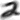
\includegraphics[scale=3]{proiettato6.png}
\quad

\includegraphics[scale=3]{proiettato10.png}
\caption{Immagine originale e proiettata in dimensione $2$, $6$ e $10$.}
\end{figure}

\end{frame}

\begin{frame}{Classificazione - Idea 1}
\begin{itemize}
\item{
$ X_{train}=[X_{train}^0,\dots , X_{train}^9]
\quad \rightarrow $\quad PCA
}
\vspace{ 6mm}\\
\item{ 
$[U_{red}(0),\dots,U_{red}(9)], \quad [\lambda ^0,\dots,\lambda^9]$
}
\vspace{ 6mm}\\
\item{
$ X_{test} \quad \rightarrow \quad [ a(0,X_{test}),\dots,a(9,X_{test}) ] 
$ }
\vspace{ 6mm}\\
\item{Idea: se $t_{test} = i \quad \rightarrow \quad a(i,X_{test})>a(j,X_{test}) \quad \textrm{per $i \neq j $}$
}

\end{itemize}

\end{frame}

\begin{frame}{Classificazione - Idea 1}
\begin{itemize}

\item{Per ogni test $X_{test}$ valutiamo le funzioni $$f_i(X_{test})=\frac{\sum_{j=1}^d \lambda_j^i a(i,X_{test})^2_j}{\sum_{j=1}^d \lambda_k^i}$$
}
\vspace{ 3mm}\\
\item{Prendo $$i=\argmax{j}f_j(X_{test})$$ come predizione del nostro modello.}
\end{itemize}

\end{frame}

\begin{frame}{Classificazione - Idea 1}
\begin{itemize}
\item{Training set molto grande $\rightarrow$ lo dividiamo in diversi training set pi� piccoli.}\vspace{ 6mm}\\
\item{Ognuno di questi fornisce una predizione sul test.} \vspace{ 6mm}\\
\item{Abbiamo implementato due metodi diversi che ottengono una predizione finale basata sulle varie predizioni precedenti.}
\end{itemize}
\end{frame}

\begin{frame}{Classificazione - Idea 1 - Davide}
\begin{itemize}
\item{La convinzione su cui si basa questo metodo � che non tutti i training set siano ugualmente buoni.}\vspace{6mm}
\item{Per validare questi set ho preso diversi validation set e di volta in volta ho scartato i training set che si comportavano peggio.
$$
\textrm{Se} \quad \frac{\textrm{cifre azzeccate dal train $j$}}{\textrm{cifre totali}}<\textrm{tol} \quad \rightarrow \quad \textrm{scarto il training set $j$}
$$ } \vspace{3mm}
\item{La \textrm{tol} l'ho fissata usando un altro validation set a $0.56$ }
\end{itemize}
\end{frame}

\begin{frame}{Classificazione - Idea 1 - Davide}
\begin{itemize}
\item{Con i training set rimasti ho usato come predizione finale la moda dei vari train.} \vspace{6mm}
\item{Cos� facendo ho ottenuto il valore ottimo di $80,05\%$ di cifre riconosciute, usando come dimensione della PCA $8$ e $24$ training set validati partendo da 100 totali, ciascuno di 1000 elementi.}
\vspace{3mm}\\
\end{itemize}
\center
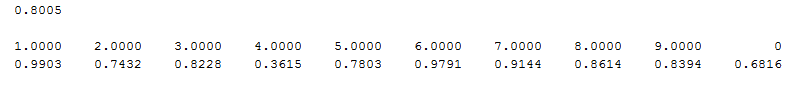
\includegraphics[scale=0.55]{alfa1davide.png}
\end{frame}

\begin{frame}{Classificazione - Idea 1 - Davide}
\begin{itemize}
\item{Per rendere il risultato confrontabile con altri (quello di Luca), ho dovuto creare una funzione probabilit� che assegni ad ogni test una probabilit� di essere assegnata alla cifra $k$.}\vspace{6mm}
\item{Perci�, invece di prendere la moda dei train, ho fatto le medie delle funzioni $f_i$ dei vari train selezionati:
$$
p(\textrm{classe } j|x)=\frac{\sum_{i=1}^{N_{train}} f_j^i(x)}{\sum_{i=1}^{N_{train}}\sum_{k=1}^{10} f_k^i(x) } .
$$ }
\end{itemize}
\end{frame}

\begin{frame}{Classificazione - Idea 1 - Luca}
\begin{itemize}
\item{L'idea � fare una media delle predizioni fornite dai vari training set.}
\vspace{ 3mm}\\
\item{Per ogni train $j$ calcolo la probabilit� che $X_{test}$ sia assegnato alla cifra $i$ come:
$$ P(X_{test}=i | \textrm{train $j$} ) = \frac{f^j_i(X_{test})}{\sum_{k=0}^9 f^j_k(X_{test})} .$$  }
\vspace{3mm}\\
\item{La predizione finale che ottengo � una probabilit� che $X_{test}$ sia assegnato alla cifra $i$, ottenuta mediando le precedenti sui vari training set:
$$  P(X_{test}=i) = \frac{1}{n_{train}} \sum_{j=1}^{n_{train}} P(X_{test}=i | \textrm{train $j$} ) .$$  }
\end{itemize}
\end{frame}

\begin{frame}{Classificazione - Idea 1 - Luca}
\begin{itemize}
\item{Altra idea: implementare un metodo che per ogni cifra non utilizzi i train set che funzionano "male" per imparare tale cifra. }\vspace{3mm}\\
\item{Si calcola, usando diversi validation set, il seguente indice:
$$ \textrm{ind}(i,j) = \begin{cases}
1 & \quad\textrm{se $ \textrm{perc}(i | \textrm{train $j$})> \textrm{tol}$ per ogni validation set}\\
0 & \quad\textrm{altrimenti}
\end{cases} \ $$ 
dove $\textrm{tol}$ � una tolleranza fissata e 
$ \textrm{perc}(i | \textrm{train $j$})$ � la percentuale di cifre $i$ azzeccate usate il $j$-esimo train.}\vspace{3mm}\\
\item{Definisco quindi $\textrm{pos}(i,j) = \inf\{k\geq1 : \sum_{l=1}^k \textrm{ind}(i,l) = j \}$.} 
\end{itemize}
\end{frame}

\begin{frame}{Classificazione - Idea 1 - Luca}
\begin{itemize}
\item{Definisco, pero ogni train $j$ e cifra $i$:
$$ l^j_i(X_{test}) = \frac{f^{\textrm{pos}(i,j)}_i(X_{test})}{\sum_k f^{\textrm{pos}(i,j)}_k(X_{test})}. $$  }
\vspace{3mm}\\
\item{Si calcola quindi infine la probabilit� che a $X_{test}$ sia associata la cifra $i$ come:
$$ P(X_{test} = i) = \frac{\sum_j l^j_i (X_{test})}{\sum_{k,j}l_k^j(X_{test})}. $$  }
\end{itemize}
\end{frame}

\begin{frame}{Classificazione - Idea 1 - Luca}
\begin{itemize}
\item{In realt�, testando i due metodi, si trova che funziona meglio il primo, ovvero quello che usa tutti i train, senza scartarli.}
\vspace{3mm}\\
\item{Con tale metodo si ottengono sui dati di test le seguenti percentuali di cifre azzeccate:}
\end{itemize}
\vspace{3mm}
\center
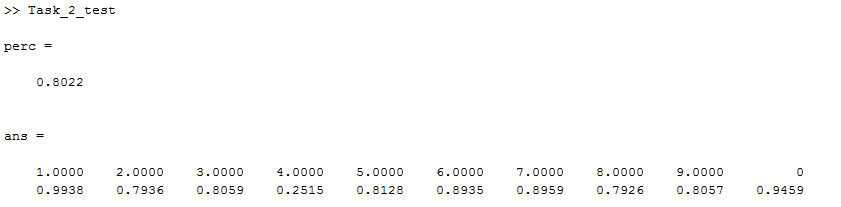
\includegraphics[scale=.55]{alpha1_luca.png}
\end{frame}

\begin{frame}{Classificazione - Idea 1 - Parametro 'Peso'}
\begin{itemize}
\item{Da entrambi i metodi risulta che alcuni numeri sono spesso misclassificati, ad esempio il 4 era la cifra peggio riconosciuta.}\vspace{3mm}
\item{Idea: pesare le $f_i$ con dei coefficienti $\alpha_i$ in modo da "favorire" le cifre peggiori:
$$ f_i^{new}(X_{test})=\alpha_i \cdot f_i(X_{test}).$$ }\vspace{3mm}
\item{Come scelgo $\alpha$?}
\end{itemize}
\end{frame}

\begin{frame}{Classificazione - Idea 1 - Davide: Parametri Ottimi}
\begin{itemize}
\item{$\alpha = [0.88,1.08,1.05,1.23,1.13,0.98,1,1.09,1.05,1.21]$.} \vspace{3mm}
\item{Percentuali di cifre azzeccate ottenute:}
\end{itemize}
\vspace{3mm}
\center
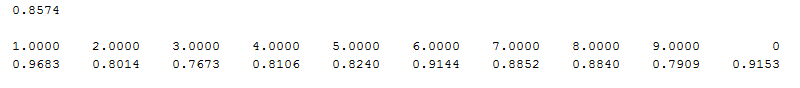
\includegraphics[scale=.55]{alfabestdavide.png}
\end{frame}

\begin{frame}{Classificazione - Idea 1 - Luca: Parametri Ottimi}
\begin{itemize}
\item{$\alpha = [1,1.07,1.05,1.25,1,1,1,1.05,1.09,1]$.} \vspace{3mm}
\item{Percentuali di cifre azzeccate ottenute:}
\end{itemize}
\vspace{3mm}
\center
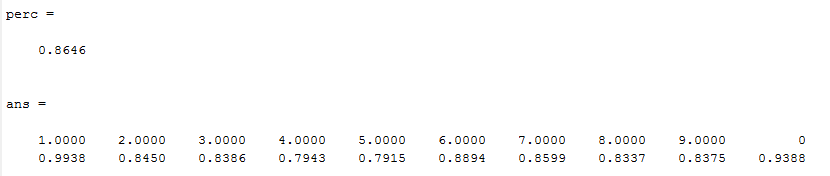
\includegraphics[scale=.55]{bestalpha_luca.png}
\end{frame}

\begin{frame}{Classificazione - Idea 1 - Osservazioni}
\begin{itemize}
\item{Mediando le probabilit� ottenute dai due metodi si ottiene una percentuale di cifre azzeccate dell'$87,37\% $.}\vspace{6mm}
\item{Abbiamo provato ad usare la funziona matlab $\texttt{fmincon}$ per cercare gli $\alpha$ migliori, ma non funzionava.}\vspace{6mm}
\item{Aumentando la dimensione del PCA oltre un certo valore, il risultato peggiora (troppo rumore?).}\vspace{6mm}
\end{itemize}
\end{frame}

\begin{frame}{Classificazione - Logistic Multiclass Regression}
\begin{itemize}
\item{L'approcio proposto finora pu� essere leggermente modificato per trasformarlo in un algoritmo di Logistic Multiclass Regression.}\vspace{3mm}
\item{Definiamo le funzioni $\Phi_i(\textbf{x}) = f_i(\textbf{x})$.}\vspace{3mm}
\item{Tale algoritmo calcola quindi le probabilit�
$$ P(C_k|\textbf{x}) = y_k(\textbf{x}) =  \frac{\exp(a_k)}{\sum_j\exp(a_j)} $$
dove $a_k = \textbf{w}_k^T\cdot \textbf{$\Phi$}(\textbf{x})$. }\vspace{3mm}
\item{Nel nostro approcio abbiamo utlizzato $\textbf{w}_k = \alpha_k \textbf{e}_k$.}
\end{itemize}
\end{frame}

\begin{frame}{Classificazione - Stochastic Gradient Descent}
\begin{itemize}
\item{Si possono calcolare i $\textbf{w}_k$ migliori andando a minimizzare la funzione:
$$ E(\textbf{w}_0,\dots,\textbf{w}_9) = - \sum_{n=1}^N \sum_{k=0}^9 t_{nk}\log(y_{nk}) $$ dove $N$ � il numero di dati di training.} \vspace{3mm}
\item{Poich� la funzione  da minimizzare � del tipo $$ f(\textbf{x}) = \sum_{n=1}^N f_n(\textbf{x}) $$ si potrebbe utilizzare un algoritmo di stochastic gradient descent per la ricerca dei minimi dividendo i train (e quindi la somma su $n$) in vari 'blocchetti'.}
\end{itemize}
\end{frame}

\begin{frame}{Classificazione - Idea 2}
\begin{itemize}
\item{Usare SVM per distinguere 2 cifre.} \vspace{12mm}
\item{Usare strategia tutti contro tutti o con scontri tra gruppi di cifre.} \vspace{12mm}
\item{Usare la PCA su tutti i dati di training con dimensioni maggiori.}
\end{itemize}
\end{frame}

\begin{frame}{Classificazione - Idea 2 - SVM: 1 vs 1}
\begin{itemize}
\item{Le percentuali di cifre ben classificate nell'1 vs 1 sono le seguenti:}
\end{itemize}
\center
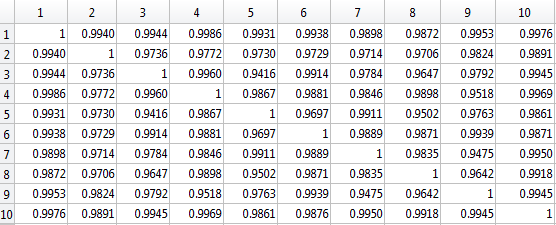
\includegraphics[scale=.7]{1vs1.png}
\end{frame}

\begin{frame}{Classificazione - Idea 2 - SVM: Torneo}
\begin{itemize}

\item{Abbiamo diviso le cifre in gruppi (tenendo conto delle misclassificazioni) e abbiamo organizzato un torneo tra gruppi di cifre per ogni test.}\vspace{6mm}
\item{1$^\circ$ Round: $[0, 1, 2, 6 ]$ vs $[3,4,5,7,8,9]$}
\item{2$^\circ$ Round: $[0, 6]$ vs $[1, 2]$ e $[3,8,5]$ vs $[4, 7,9]$}
\item{3$^\circ$ Round: $[0]$ vs $[6]$ e $[1]$ vs $[2]$ e $[3,5]$ vs $[8]$ e $[4]$ vs $[7,9]$}
\item{4$^\circ$ Round: $[3]$ vs $[5]$ e $[7]$ vs $[9]$} \vspace{6mm}
\item{Il risultato migliore ottenuto fornisce $85,63\%$ cifre azzeccate, con dimensione del PCA $45$.}  

\end{itemize}

\end{frame}

\begin{frame}{Classificazione - Idea 2 - SVM: Tutti contro tutti}
\begin{itemize}
\item{Un'altra strategia provata � quella di confrontare per ogni test, ciascuna cifra contro l'altra.}\vspace{6mm}
\item{Per ogni test, si sceglie quindi la cifra che ha vinto pi� partite contro le altre 9.}\vspace{6mm}
\item{I risultati ottenuti con questa strategia arrivano a riconoscere il $94,04\%$ di cifre, con dimensione del PCA $60$.} \vspace{6mm}
\item{Aumentando la dimensione i risultati migliorano leggermente ma i costi computazionali si alzano.}

\end{itemize}
\end{frame}

\begin{frame}{Classificazione - Idea 2 - SVM: Tempi}
\begin{itemize}
\item{Interessante notare che i tempi impiegati per fare SVM durante gli scontri tra le diverse coppie di cifre sono molto diversi: passano da un minimo di circa $1$ secondo a un massimo di $25$ secondi.}
\end{itemize}
\center
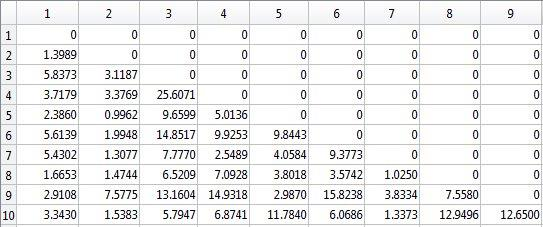
\includegraphics[scale=0.7]{time_svm.jpg}

\end{frame}

\begin{frame}{Classificazione - Osservazioni finali}
\begin{itemize}
\item{Le cifre di training e test sono brutte e di bassa qualit�.}\vspace{6mm}
\item{Se avessimo dei pixel in pi� probabilmente funzionerebbe meglio (in rete si trovano soprattutto esempi di $28\times 28$ pixel).}\vspace{6mm}
\item{Per implementare un software di riconoscimento cifra, bisogna anche aggiungere un preprocessing che centri l'immagine e la ingrandisca sui pixel interessanti.}\vspace{6mm}
\item{Google inoltre usa l'informazione della direzione in cui si sta scrivendo.}\vspace{6mm}

\end{itemize}
\end{frame}

\begin{frame}{Classificazione - Testiamo i metodi!}
\begin{itemize}
\item{\href{run:C:/Users/Luca/Documents/MATLAB/Statistica Computazionale/Progetto_Task_2_Luca/Try/prova.png}{Draw!}}
\end{itemize}
\end{frame}

\end{document}


